\newpage

\subsection{Patterns}
Patterns, sogenannte Entwurfsmuster, wurden ursprünglich vom Architekten Christopher Alexander geprägt.
Dieser beschrieb in seinem Buch \enquote{A Pattern Language: Towns, Buildings, Construction}\cite{a-pattern-language} im Jahr 1977 zum ersten Mal Muster, unter dessen Einsatz sich wiederkehrende Probleme lösen lassen.
In der Informatik wurden Entwurfsmuster durch die Veröffentlichung der \enquote{Gang of Four} im Jahr 1994 populärer.
In ihrem Buch \enquote{Design Patterns - Elements of Reusable Object-Oriented Software}\cite{gamma-design-patterns} beschreiben Erich Gamma et al.\ 23 unterschiedliche Entwurfsmuster.
Diese sind eingeteilt in die drei Kategorien Creational, Structural und Behavioral.

1999 ergänzte Martin Fowler in \enquote{Patterns of Enterprise Application Architecture}\cite{patterns-of-enterprise-application-architecture} die Kategorie \enquote{Objektrelationale Abbildung} und dazugehörige Muster.
Gregor Hohpe und Bobby Woolf ergänzten 2003 die Kategorie der Messaging Patterns in ihrem Buch \enquote{Enterprise Integration Patterns}\cite{enterprise-integration-patterns}.

Die Menge der Entwurfsmuster ist sehr umfangreich, weshalb im Folgenden nur jene Muster skizziert werden, die im anschließenden Vergleich verwendet werden.

\subsubsection{MVC (Model-View-Controller)}
Dieses architektonische Pattern teilt eine interaktive Anwendung in drei Komponenten auf.
Durch eine klare Trennung der Zuständigkeiten werden Wartungen einfacher und können besser auf unterschiedliche Entwickler aufgeteilt werden.
Das Model ist nur zuständig für Daten und Business Logic, die View hingegen, nur für die Darstellung der Inhalte (\ref{fig:mvc}).
Der Controller ist das Bindeglied und routet Daten sowie Befehle zwischen den beiden anderen Bereichen.
(Vgl.~\cite{buschmann-pattern-oriented-software-architecture})

\begin{figure}[h!]
    \centering
    \caption{Model View Controller}
    \label{fig:mvc}
    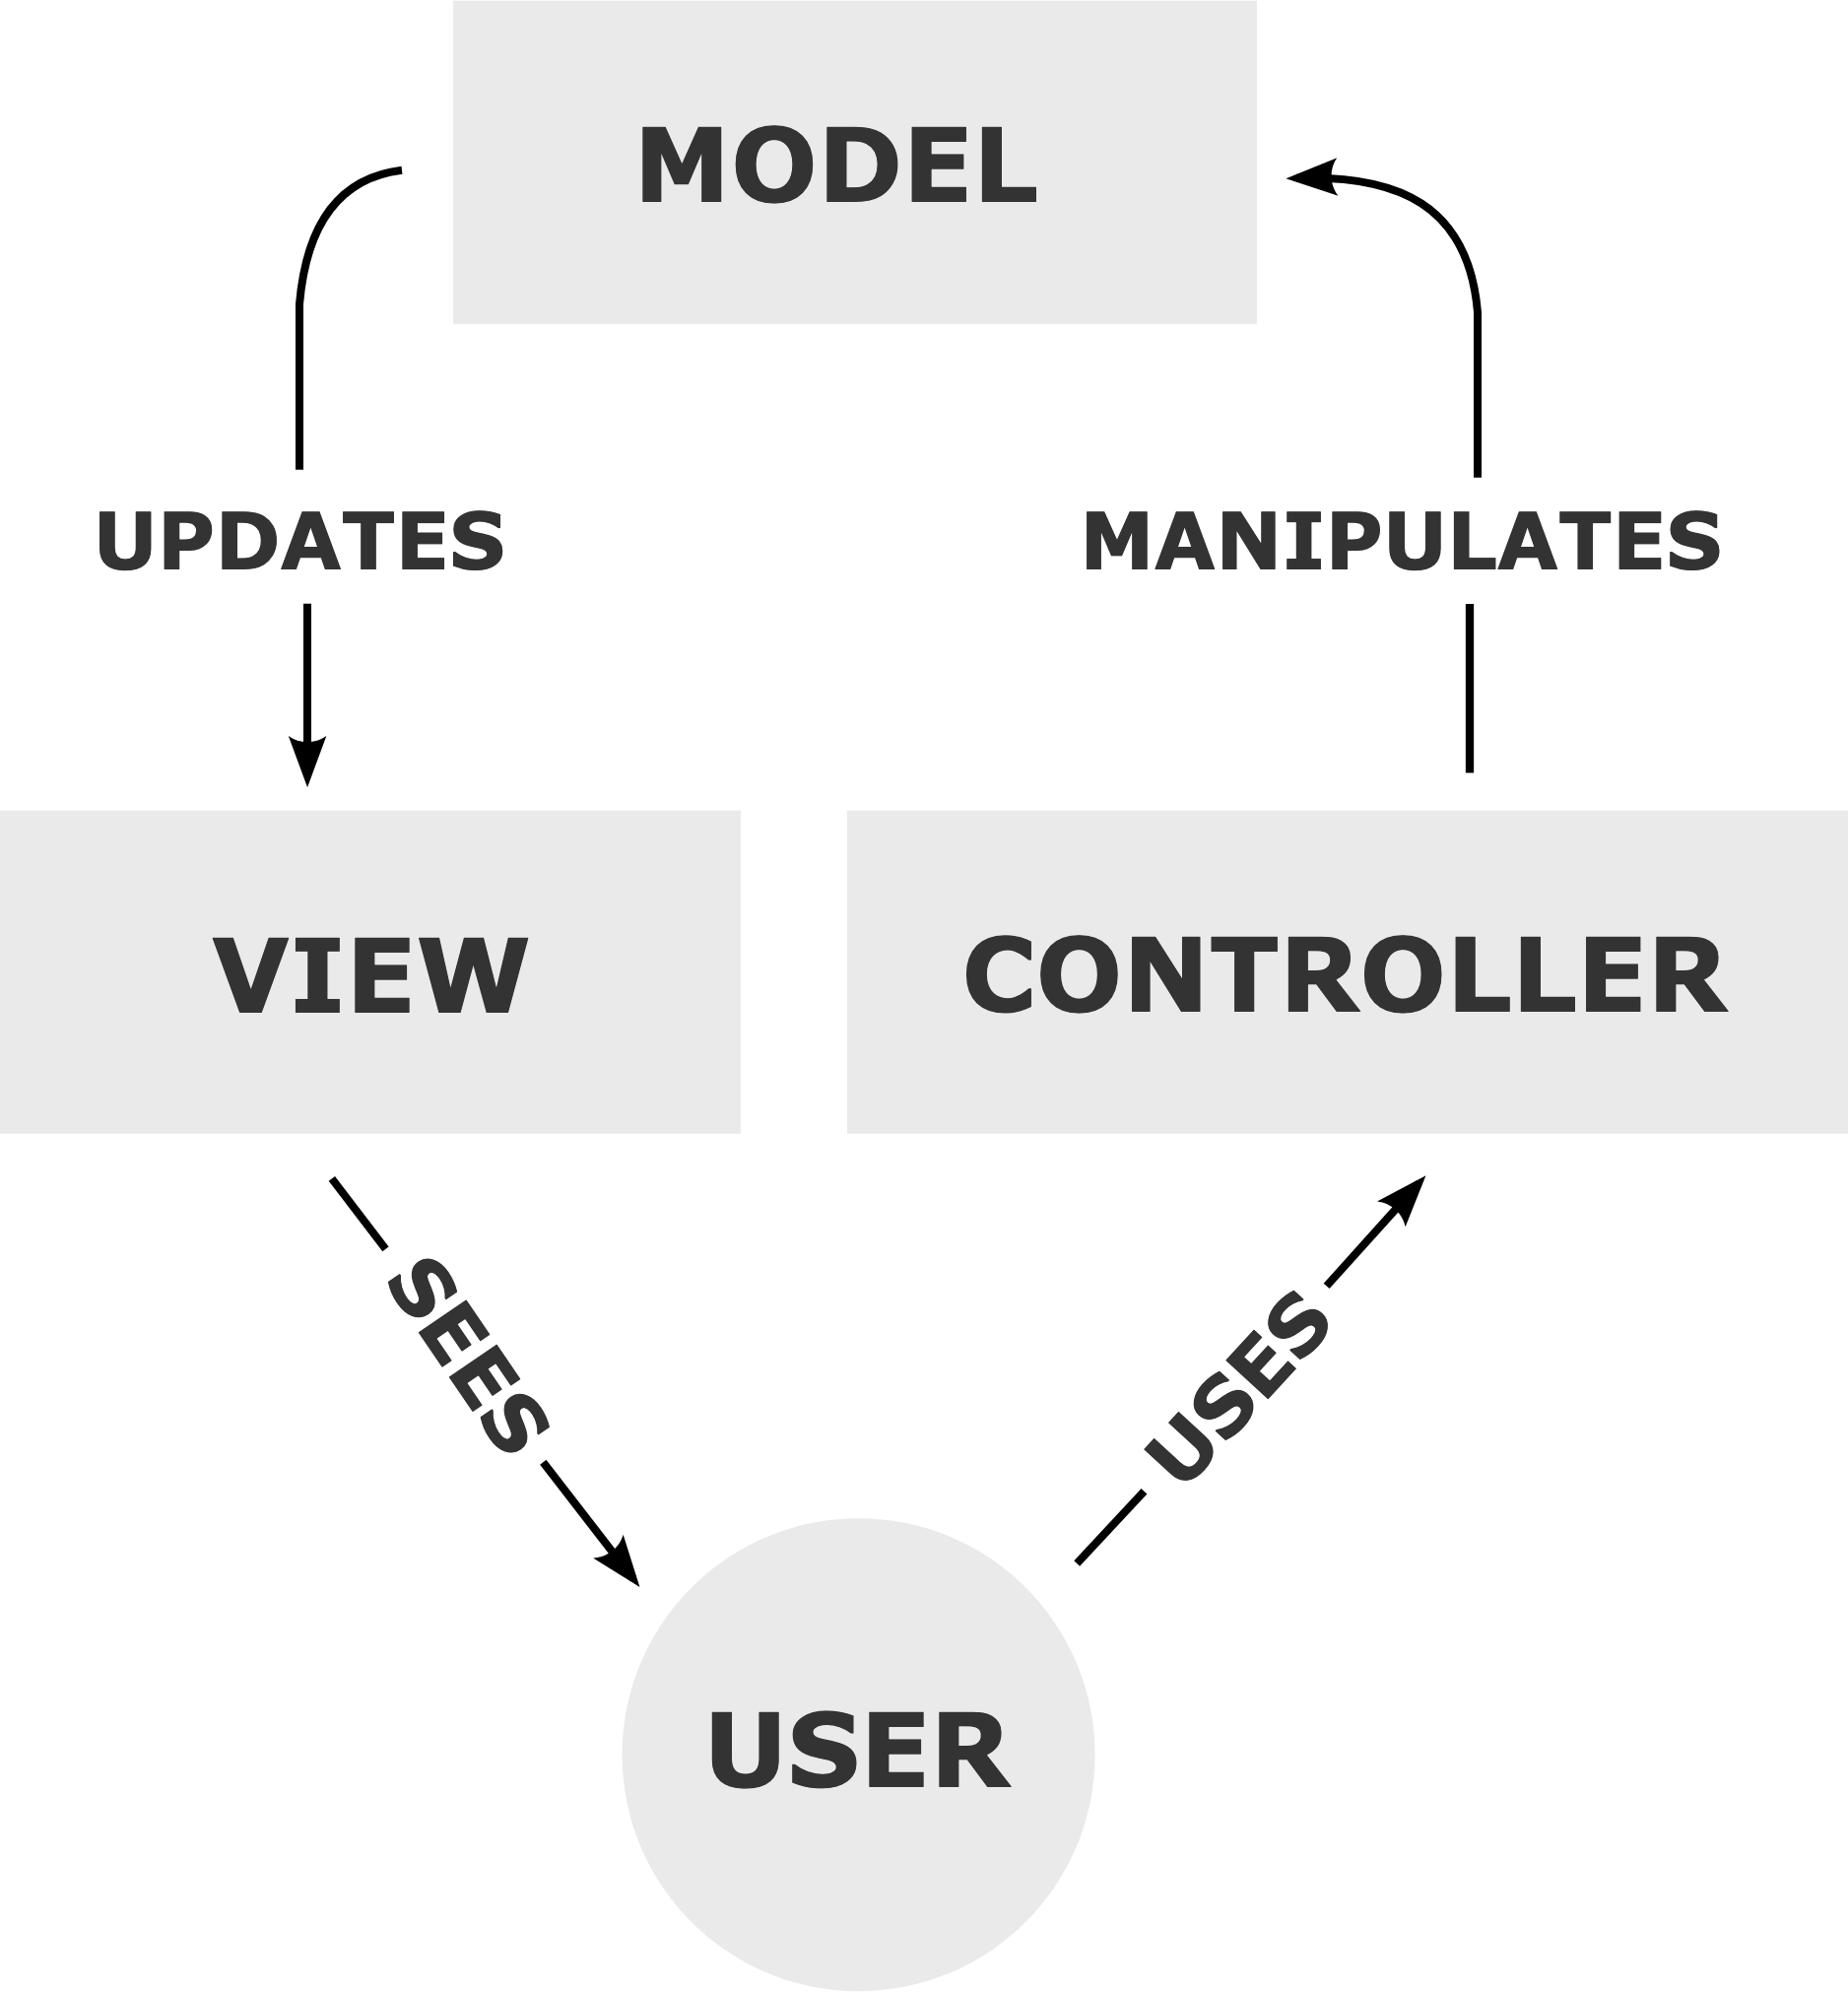
\includegraphics[scale=0.20]{assets/wikipedia_mvc_process}
\end{figure}

\subsubsection{PAC (Presentation-Abstraction-Control)}
Dieses Pattern definiert eine hierarchische Struktur aus kooperierenden Agenten für interaktive Softwaresysteme.
Jeder Agent ist für einen Aspekt der Anwendung zuständig und besteht aus drei Komponenten: Presentation, Abstraction und Control.
Auf diese Weise wird die Präsentationsebene, mit der Menschen interagieren, vom Funktionskern der Anwendung und der Kommunikation mit anderen Komponenten getrennt.

(Vgl.~\cite{buschmann-pattern-oriented-software-architecture})

\subsubsection{View Handler}
Wenn mehrere Ansichten in einer Anwendung benötigt werden, kann das View Handler Pattern eingesetzt werden.
Ansichten öffnen, verändern und schließen wird durch den View Handler organisiert.
Ebenso werden Abhängigkeiten zwischen den unterschiedlichen Ansichten und deren Update durch den View Handler geregelt.
Von Vorteil ist die einheitliche Handhabung der Komponenten, sowie die Erweiterbarkeit und Anpassbarkeit der Ansichten.
(Vgl.~\cite{buschmann-pattern-oriented-software-architecture})

\subsubsection{Whole-Part}
Dieses Pattern kommt zum Einsatz, wenn mehrere Komponenten eine semantische Einheit bilden können.
Es wird eine aggregierte Komponente gebildet, die ihre Bestandteile umschließt, deren Interaktion organisiert und ein Interface nach Außen abbildet.
Der direkte Zugriff auf die Bestandteile ist nicht möglich, jede Funktion wird über das \enquote{Whole} aufgerufen.
Von Vorteil ist die verbesserte Anpassbarkeit der Bestandteile der Komponenten, da jegliche Interaktion nach Außen über das Whole läuft.
Außerdem werden die einzelnen Angelegenheiten voneinander getrennt und sowohl die Wiederverwendbarkeit der Bestandteile, als auch die der Gruppe wird verbessert.
(Vgl.~\cite{buschmann-pattern-oriented-software-architecture})

\subsubsection{Layers}
Wenn die Unteraufgaben einer Applikation in unterschiedlichen Abstraktionsebenen liegen, so kann man die Applikation in Layers (übersetzt: Ebenen) aufteilen.
Ein Layer interagiert immer nur mit dem direkt untergeordneten Layer.
Für den nächsten übergeordneten Layer werden Dienste bereitgestellt.
Von Vorteil ist, dass Abhängigkeiten in der Regel nur in einem Layer liegen.
Ebenso positiv ist die Wiederverwendbarkeit, Standardisierbarkeit und Austauschbarkeit einzelner Ebenen.
(Vgl.~\cite{buschmann-pattern-oriented-software-architecture})

\subsubsection{Publisher-Subscriber}
Wenn mehrere Komponenten von Veränderungen einer anderen Komponente abhängen, kann dieses Pattern angewendet werden.
Komponenten können die Änderungen einer oder mehrerer anderer Komponenten abonnieren.
Der Publisher speichert eine Liste aller seiner Subscriber.
Im Falle eines Updates benachrichtigt er diese über Art und Inhalt der Veränderungen.
(Vgl.~\cite{buschmann-pattern-oriented-software-architecture})

\subsubsection{Broker}
Liegen in einem System unabhängige aber kooperierende Komponenten vor, so kann man diese mittels eines Brokers koppeln.
Der Broker koordiniert die Kommunikation zwischen den einzelnen Komponenten.
So leitet er Anfragen weiter und überträgt Ergebnisse und Fehlermeldungen.
Von Vorteil ist, dass anfragende Komponenten nicht wissen müssen, wo und wie sie Dienste erreichen und vice versa.
Ebenso können Komponenten einfach ausgetauscht oder erweitert werden, sofern die grundsätzliche Schnittstelle bestehen bleibt.
Zusätzlich wird die Wiederverwendbarkeit der Komponenten gestärkt.
(Vgl.~\cite{buschmann-pattern-oriented-software-architecture})

\subsubsection{Proxy}
Ein Proxy ist verantwortlich für die Kommunikation von einer oder mehrere Komponenten mit mehreren Clients.
Jegliche Kommunikation läuft repräsentativ über den Proxy, sowohl eingehende Antworten als auch ausgehende Daten.
Dies kann die Effizienz steigern, den Zugriff vereinfachen und den Zugriff steuern.
Ebenso können die Komponenten hinter dem Proxy besser angepasst werden, ohne dass Anpassungen an den Clients notwendig werden.
(Vgl.~\cite{buschmann-pattern-oriented-software-architecture})
